
\begin{appendices}

\chapter*{\textsc{Annexe A}}
	\addcontentsline{toc}{chapter}{\textsc{Annexe A}}		
	
	\label{Annexe A} \hyperref[section 2.2.2]{Retour vers section 2.2.2}
	
	\subsection{Visualisation}

	\begin{center}
	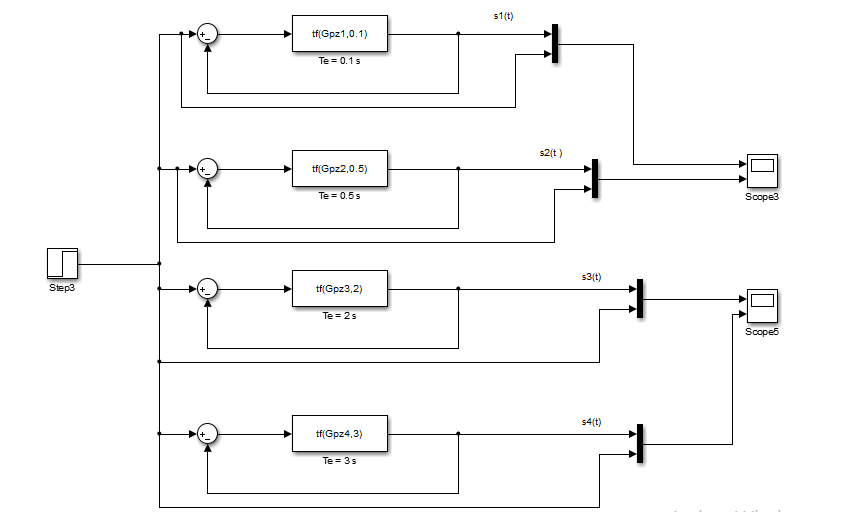
\includegraphics[scale=0.5]{shem1.png}
	\captionof{figure}{\textit{Schema simulink du système échantillonné pour différentes valeurs de $T_e$ \\}}
	\label{fig4} 
	\end{center}
	
	\begin{center}
	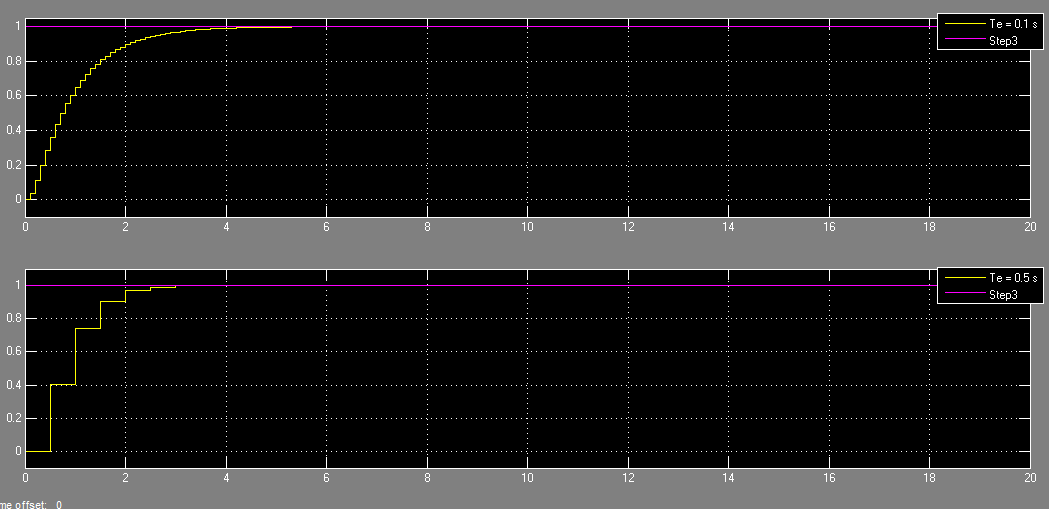
\includegraphics[scale=0.4]{simu1.png}
	\captionof{figure}{\textit{Réponses simulink de $s(t)$ pour de $T_e=0.1s$ et $T_e=0.5s$ \\}}
	\label{fig5} 
	\end{center}
	
	\begin{center}
	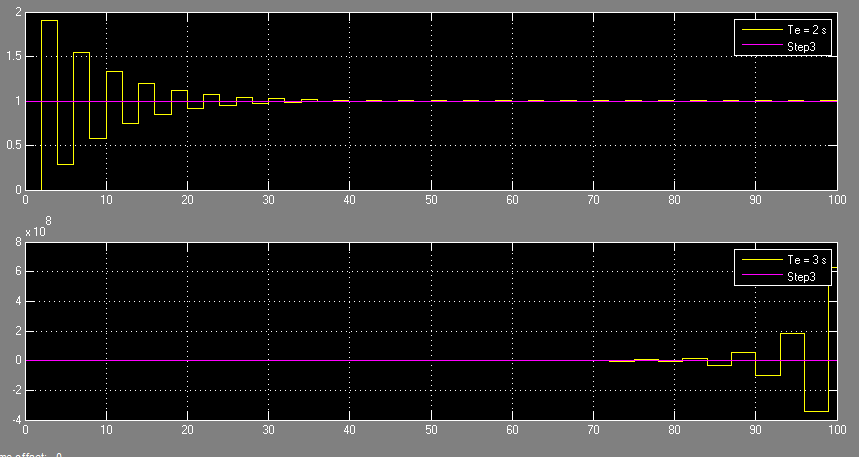
\includegraphics[scale=0.5]{simu2.png}
	\captionof{figure}{\textit{Réponses simulink de $s(t)$ pour de $T_e=2s$ et $T_e=3s$ \\}}
	\label{fig6} 
	\end{center}
	
\subsection{Commentaires}

\par Le système diverge pour $T_e = 3 s$, il possède plusieurs oscillations et tarde à ce converger pour $T_e = 2 s$ donc ces deux cas seront écartés.\\

   	
	\begin{center}
	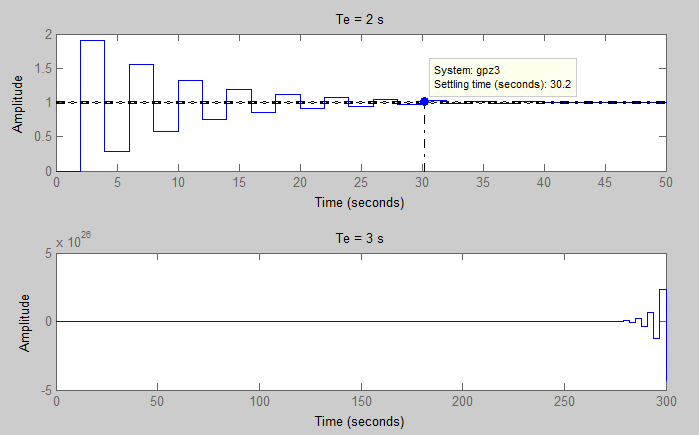
\includegraphics[scale=0.5]{mat2.png}
	\captionof{figure}{\textit{Réponses $s(t)$ pour de $T_e=2s$ et $T_e=3s$ \\}}
	\label{fig7} 
	\end{center}

Il nous reste à comparer entre la réponse à $T_e=0.1s$ et à  $T_e=0.5s$, comparons leurs temps de réponses respectifs:\\
   
   	
	\begin{center}
	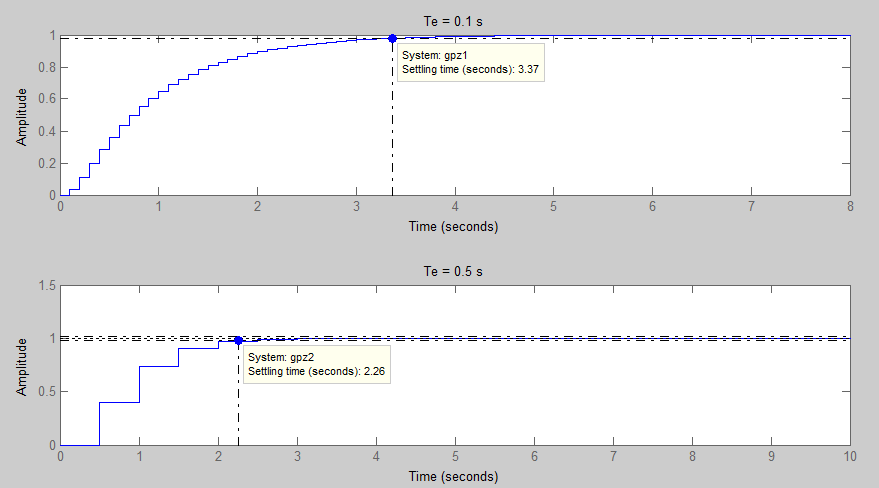
\includegraphics[scale=0.5]{mat1.png}
	\captionof{figure}{\textit{Réponses $s(t)$ pour de $T_e=0.1s$ et $T_e=0.5s$ \\}}
	\label{fig8} 
	\end{center}
	
\par Il est clair qu'on écartera l'échantillonnge à $T_e=0.1$ et on retiendra celui à $T_e=0.5$ car le premier ne respecte pas le temps de réponse que possède le système en temps continu contrairement à l'échantillonnage à $T_e=0.5 $ qui possède un temps de réponse $t_r = 2.26 s$ et ne possède pas de dépassement,alors il respecte toutes les performances du système en temps continu.\\ 	

\chapter*{\textsc{Annexe B}}
	\addcontentsline{toc}{chapter}{\textsc{Annexe B}}	
	\par Code Matlab.\\
	\begin{lstlisting}
	
clc
clear all
close all
t=0.1;
Kg=1;
G=tf([Kg],[t 1 0]);


Gbf=feedback(G,1);

% figure(1)
% margin(G)
% grid
% 
% figure(2)
% step(Gbf)
%   
% margin(Gbf)
% grid
T=feedback(G,1);
S=1-T;
pole(T)



Gpz1=c2d(G,0.1,'zoh')
gpz1=feedback(Gpz1,1);
% 
Gpz2=c2d(G,0.5,'zoh')
gpz2=feedback(Gpz2,1);
% 
Gpz3=c2d(G,2,'zoh')
gpz3=feedback(Gpz3,1);
 
Gpz4=c2d(G,3,'zoh')
gpz4=feedback(Gpz4,1);


figure(3)
subplot(2,1,1)
step(gpz1 )
title('Te = 0.1 s')

subplot(2,1,2)
step(gpz2)
title('Te = 0.5 s')


figure(4)
subplot(2,1,1)
step(gpz3)
title('Te = 2 s')

subplot(2,1,2)
step(gpz4)
title('Te = 3 s')


%rltool(Gpz2)

figure(5)
eig(feedback(6.60775*Gpz2,1))
eig(feedback(0.000000000000000000000000001*Gpz2,1))
%pour Te=0.5
b1=0.006738;
a1=0.40067;
a=0.8;
%a0=0;
%a=0.02;
a2=0.2395;
C1=zpk([a b1],[1 -a2],[1],0.5);
Bo=C1*Gpz2;
BoBF=feedback(Bo,1);
step(BoBF)
title('a = 0.8')

figure(6)
subplot(2,1,1)
rlocus(Bo)
title('a1 = 0.40067')
subplot(2,1,2)
Bo1=C1*Gpz2*100;
rlocus(Bo1)
title('a1 = 0.40067*100')
	
	\end{lstlisting}
	
\end{appendices}	